%% LyX 2.0.3 created this file.  For more info, see http://www.lyx.org/.
%% Do not edit unless you really know what you are doing.
\documentclass[10pt]{beamer}\usepackage[]{graphicx}\usepackage[]{color}
%% maxwidth is the original width if it is less than linewidth
%% otherwise use linewidth (to make sure the graphics do not exceed the margin)
\makeatletter
\def\maxwidth{ %
  \ifdim\Gin@nat@width>\linewidth
    \linewidth
  \else
    \Gin@nat@width
  \fi
}
\makeatother

\definecolor{fgcolor}{rgb}{0.345, 0.345, 0.345}
\newcommand{\hlnum}[1]{\textcolor[rgb]{0.686,0.059,0.569}{#1}}%
\newcommand{\hlstr}[1]{\textcolor[rgb]{0.192,0.494,0.8}{#1}}%
\newcommand{\hlcom}[1]{\textcolor[rgb]{0.678,0.584,0.686}{\textit{#1}}}%
\newcommand{\hlopt}[1]{\textcolor[rgb]{0,0,0}{#1}}%
\newcommand{\hlstd}[1]{\textcolor[rgb]{0.345,0.345,0.345}{#1}}%
\newcommand{\hlkwa}[1]{\textcolor[rgb]{0.161,0.373,0.58}{\textbf{#1}}}%
\newcommand{\hlkwb}[1]{\textcolor[rgb]{0.69,0.353,0.396}{#1}}%
\newcommand{\hlkwc}[1]{\textcolor[rgb]{0.333,0.667,0.333}{#1}}%
\newcommand{\hlkwd}[1]{\textcolor[rgb]{0.737,0.353,0.396}{\textbf{#1}}}%
\newcommand\myeq{\stackrel{\mathclap{\normalfont\mbox{d}}}{=}}



\usepackage{fontawesome5}
\usepackage{amsmath}
\usepackage{amssymb}
\usepackage{framed}
\makeatletter
\newenvironment{kframe}{%c
 \def\at@end@of@kframe{}%
 \ifinner\ifhmode%
  \def\at@end@of@kframe{\end{minipage}}%
  \begin{minipage}{\columnwidth}%
 \fi\fi%
 \def\FrameCommand##1{\hskip\@totalleftmargin \hskip-\fboxsep
 \colorbox{shadecolor}{##1}\hskip-\fboxsep
     % There is no \\@totalrightmargin, so:
     \hskip-\linewidth \hskip-\@totalleftmargin \hskip\columnwidth}%
 \MakeFramed {\advance\hsize-\width
   \@totalleftmargin\z@ \linewidth\hsize
   \@setminipage}}%
 {\par\unskip\endMakeFramed%
 \at@end@of@kframe}
\makeatother

\definecolor{shadecolor}{rgb}{.97, .97, .97}
\definecolor{messagecolor}{rgb}{0, 0, 0}
\definecolor{warningcolor}{rgb}{1, 0, 1}
\definecolor{errorcolor}{rgb}{1, 0, 0}
\newenvironment{knitrout}{}{} % an empty environment to be redefined in TeX

\usepackage{alltt}
\usepackage[T1]{fontenc}
\setcounter{secnumdepth}{3}
\setcounter{tocdepth}{3}
\usepackage{tikz}
\usepackage{color}
\usepackage{colortbl}
\usepackage{dcolumn}
\usepackage{amsmath}
\usepackage{tikz}
\usepackage{floatflt}
\usepackage{multicol}
\usepackage{multirow}
\usepackage{listings}
\usepackage{tabularx}
\usepackage{amssymb}% http://ctan.org/pkg/amssymb
\usepackage{pifont}% http://ctan.org/pkg/pifont
\usepackage{bbm}
\usepackage{siunitx}
\usepackage{url}
\usepackage{verbatim}
\usepackage{enumerate}
\usepackage{algorithmic}
\usepackage{algorithm}
\usepackage{algpseudocode}
\usepackage[flushleft]{threeparttable}
\usepackage{amsfonts}
\usepackage{booktabs}
\usepackage{graphicx}
\usepackage{siunitx}

\usepackage{hyperref}
\hypersetup{
    colorlinks=magenta,
    linkcolor=blue,
    filecolor=magenta,      
    urlcolor=magenta
     }
     
    \definecolor{links}{HTML}{2A1B81}
\hypersetup{colorlinks,linkcolor=blue, urlcolor=magenta}


\makeatletter

%%%%%%%%%%%%%%%%%%%%%%%%%%%%%% LyX specific LaTeX commands.
\providecommand{\LyX}{\texorpdfstring%
  {L\kern-.1667em\lower.25em\hbox{Y}\kern-.125emX\@}
  {LyX}}


%%%%%%%%%%%%%%%%%%%%%%%%%%%%%% Textclass specific LaTeX commands.
 % this default might be overridden by plain title style
 \newcommand\makebeamertitle{\frame{\maketitle}}%
 \AtBeginDocument{
   \let\origtableofcontents=\tableofcontents
   \def\tableofcontents{\@ifnextchar[{\origtableofcontents}{\gobbletableofcontents}}
   \def\gobbletableofcontents#1{\origtableofcontents}
 }
 \def\lyxframeend{} % In case there is a superfluous frame end
 \long\def\lyxframe#1{\@lyxframe#1\@lyxframestop}%
 \def\@lyxframe{\@ifnextchar<{\@@lyxframe}{\@@lyxframe<*>}}%
 \def\@@lyxframe<#1>{\@ifnextchar[{\@@@lyxframe<#1>}{\@@@lyxframe<#1>[]}}
 \def\@@@lyxframe<#1>[{\@ifnextchar<{\@@@@@lyxframe<#1>[}{\@@@@lyxframe<#1>[<*>][}}
 \def\@@@@@lyxframe<#1>[#2]{\@ifnextchar[{\@@@@lyxframe<#1>[#2]}{\@@@@lyxframe<#1>[#2][]}}
 \long\def\@@@@lyxframe<#1>[#2][#3]#4\@lyxframestop#5\lyxframeend{%
   \frame<#1>[#2][#3]{\frametitle{#4}#5}}

\renewcommand{\footnotesize}{\fontsize{6pt}{6pt}\selectfont}

% Redefine footnote numbering to use symbols
\makeatletter
\renewcommand{\thefootnote}{\alph{footnote}}
\makeatother


\newcommand{\indep}{\rotatebox[origin=c]{90}{$\models$}}

% https://dkumor.com/posts/technical/2018/08/15/causal-tikz/

% Tikz settings optimized for causal graphs.
% Just copy-paste this part
\usetikzlibrary{shapes,decorations,arrows,calc,arrows.meta,fit,positioning}
\tikzset{
    -Latex,auto,node distance =1 cm and 1 cm,semithick,
    state/.style ={ellipse, draw, minimum width = 0.7 cm},
    point/.style = {circle, draw, inner sep=0.04cm,fill,node contents={}},
    bidirected/.style={Latex-Latex,dashed},
    el/.style = {inner sep=2pt, align=left, sloped}
}


%%%%%%%%%%%%%%%%%%%%%%%%%%%%%% User specified LaTeX commands.
%\usetheme{Warsaw}
\usetheme{Boadilla}
%\setbeamertemplate{navigation symbols}{}
%gets rid of bottom navigation bars
%\setbeamertemplate{footline}[page number]{}
%\setcounter{page}{44}
%\setbeamertemplate{footline}{}

%gets rid of bottom navigation bars
\setbeamertemplate{footline}[frame number]{}

%gets rid of navigation symbols
\setbeamertemplate{navigation symbols}{}

\makeatother
\IfFileExists{upquote.sty}{\usepackage{upquote}}{}

\begin{document}


\title[Personalization]{Heterogenous Benefit/Harm Effects from Treatment}
\author[Leo Guelman]{Leo Guelman}
%\institute[RBC Royal Bank]{Head Statistician, DNA \\ RBC Royal Bank}
\date[June 2024]
{}
\makebeamertitle

\lyxframeend{}

%%%%Slide

\begin{frame}
[fragile]\frametitle{Motivation for Personalized Decision-Making}

% This is Ronald Fisher, he was a statistician and probably one of the most relevant figures in 20th century statistics 
% He's been probably most famous for his contribution to experimental design (a.k.a. A/B testing).
% He was the first to propose randomization in experiments as mechanism to eliminate confounding bias, and be able to disentangle causal relationships
% To this day A/B testing (or RCTs in clinical trials) is considered the Gold Standard to learn causal relationships in Clinical Trials and Marketing.

%\begin{figure}[t]
%\includegraphics[width=3cm]{figures/fisher.jpg}
%\caption{Ronald Fisher (1890-1962)}
%\centering
%\end{figure}



\begin{columns}[T] % align columns
\begin{column}{.48\textwidth}

\vskip25pt

\small{

\begin{itemize}

\item Personalization is founded on the premise that individuals have heterogeneous responses to actions.
% the optimal action for person A and person B might be different. 

\vskip7pt

\item Personalization algorithms aim to improve decision-making by identifying and exploiting this heterogeneity.

\end{itemize}
}


\end{column}%
\hfill%


\begin{column}{.48\textwidth}


\begin{figure}[t]
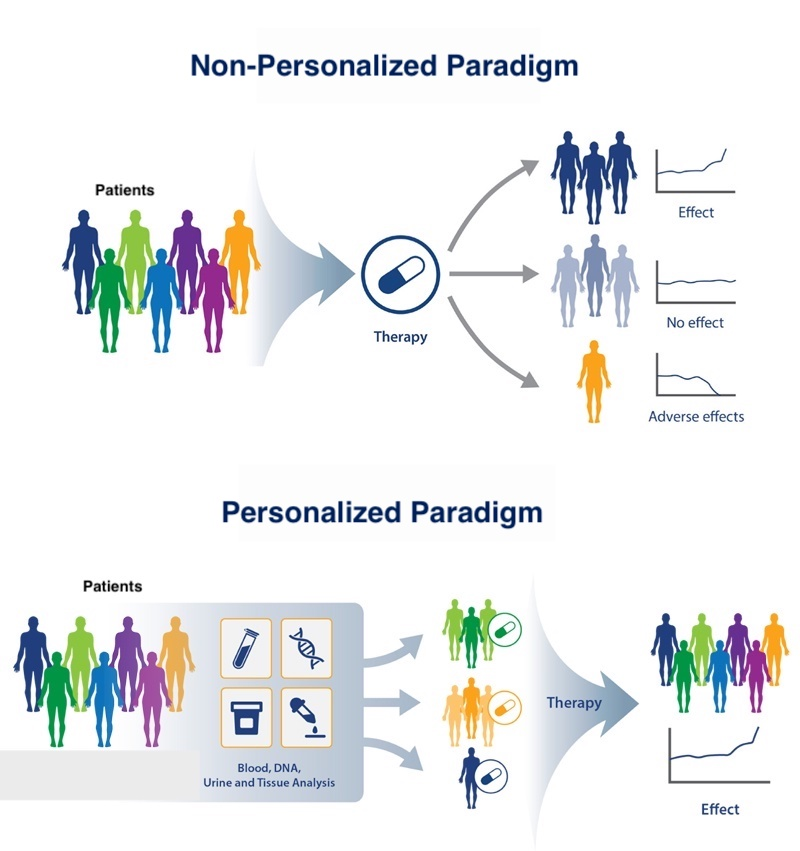
\includegraphics[width=5cm]{figures/personalizedmedv3.jpg}
\centering
\end{figure}


\end{column}%
\end{columns}


\end{frame}


%%%%Slide

\begin{frame}
[fragile]\frametitle{}

\begin{itemize}

\item Main ambition of personalized decision-making $\Rightarrow$ Achieve \textbf{subject-level} causal effect estimation.

\vskip10pt

\item Primary focus has been on methods that estimate the \textbf{Conditional Average Treatment Effects} (CATE).

\vskip10pt


\item CATE estimation can be useful, but does not imply the effects hold at the individual-level.

\vskip10pt

\item  \textbf{Individual Treatment Effects} (ITEs) are generally non-identifiable, but informative bounds can be obtained on $P(\text{ITE})$.

\vskip10pt

\item \textbf{Today's Goal}: Demonstrate how $P(\text{ITE})$ bounds can potentially help improve personalized intervention decisions, relative to using CATE.


\end{itemize}

%\begin{figure}[t]
%\includegraphics[width=3cm]{figures/fisher.jpg}
%\caption{Ronald Fisher (1890-1962)}
%\centering
%\end{figure}

\end{frame}



%%%%Slide

{
\setbeamercolor{background canvas}{bg=black}
\begin{frame}
\begin{center}

\Large{\textcolor{white}{Background}}


\end{center}
\end{frame}
}



%%%%Slide

\begin{frame}
[fragile]\frametitle{Causality has two faces: Necessary and Sufficient}

\pause

\underline{Probability of Necessity}

\vskip10pt

\begin{align*} 
PN & \triangleq P(Y_{t'} = \text{false} | T =\text{true}, Y = \text{true}) \\
 & \triangleq P(y'_{t'}  | t , y ) \\
\end{align*}

\vskip20pt

\pause

\textbf{Example}: A client got a rate discount and renewed her RBC Home Insurance policy. What is the probability she would not have renewed the policy in the absence of the discount? 


\end{frame}

%%%%Slide

\begin{frame}

\underline{Probability of Sufficiency}

\vskip10pt

\begin{align*} 
PS & \triangleq P(y_{t}  | t' , y' ) \\
\end{align*}

\vskip20pt

\pause

\textbf{Example}: A client neither got a rate discount nor renewed the insurance policy. What is the probability he would have renewed the policy with the discount? 


\end{frame}


%%%%Slide

\begin{frame}


\vskip20pt

\underline{Probability of Necessity and Sufficiency}


\begin{align*} 
PNS & \triangleq P(y_{t}, y'_{t'}) \\
  & \triangleq  P(\text{benefit}).\\
\end{align*}


\pause


\begin{itemize}

\item \textbf{Example}: What is the probability of a client renewing with rate discount and not renewing without it?

\pause

\vskip10pt

\item PNS interventions are most relevant in business settings: outcome would not occur without the intervention, and are strong enough to bring the outcome. 

\end{itemize}

\end{frame}

%%%%Slide

\begin{frame}
[fragile]\frametitle{PNS relation with CATE and ITE}

\pause
\vskip10pt

\textbf{1. PNS and ITE}

\begin{equation*}
\text{ITE} = y_t - y_{t'} 
\end{equation*}

\pause

\begin{equation*}
\text{ITE} = \begin{cases}
~~1, &   P(y_t, y'_{t'}) \\
~~0, & P(y_{t'}, y_{t}) + P(y'_{t'}, y'_{t}) \\
-1, & P(y_{t'}, y'_{t}).
\end{cases}
\end{equation*}

\pause 

\vskip20pt

Hence, PNS $\triangleq$  $P$(benefit) = $P$(ITE > 0).

\end{frame}



%%%%Slide

\begin{frame}
[fragile]\frametitle{}

\vskip10pt

\textbf{2. PNS and CATE}


\begin{align*}
\action<+-> {\text{CATE} &= P(y_t|X) -  P(y_{t'}|X)\\ }
  \action<+->{                  &= P(y_t, y'_{t'}|x) + P(y_t, y_{t'}|x) - \big( P(y_{t'}, y'_{t}|x)  +   P(y_{t'}, y_{t}|x)  \big) \\}
 \action<+->{                    &= \underbrace{P(y_t, y'_{t'}|x)}_{\text{PNS}~ \triangleq~  \text{P(benefit|x)}} - ~\underbrace{P(y_{t'}, y'_{t}|x)}_{\text{P(harm|x)}}. \\}
\end{align*}

\pause

\textbf{Remarks}

\small{
\begin{itemize}
\item $P$(harm|x) = 0 (Monotonicity) $\Rightarrow$ CATE = $P$(benefit|x).
\item Decomposing CATE into $P$(benefit|x) \text{and} $P$(harm|x) provides additional information
\begin{itemize}
\item E.g., An intervention may have the same CATE on different client groups, but different $P$(benefit|x) \text{and} $P$(harm|x) profiles. 
\end{itemize}
\item Unlike $P$(benefit|x), CATE is estimable from experimental data without invoking counterfactual expressions.
\end{itemize}
}


\end{frame}


%%%%Slide

{
\setbeamercolor{background canvas}{bg=black}
\begin{frame}
\begin{center}

\large{\textcolor{white}{Under non-monotonicity, identifying heterogenous benefit/harm effects can be more informative to conventional HTE~(CATE) to inform personalized interventions.}}


\end{center}
\end{frame}
}


%%%%Slide

\begin{frame}
[fragile]\frametitle{Toy example: Home Insurance renewal}


\begin{itemize}

\item The Home Insurance product team is aiming to send policy renewal e-mail reminders to clients. 

\vskip10pt

\item The notification is expected to increase renewal rates through early awareness. 

\vskip10pt

\pause

\item They run an A/B Test to assess the validity of this claim:

\end{itemize}

\vskip20pt

\small{

\begin {table}
\begin{center}
\begin{tabular}{ l c c c c }
 \toprule
   & Renewed & $\neg$Renewed & Total & Renewal Rate\\ 
 \toprule
do(email) & 4895 & 5105   &  10000  &  49\% \\
do($\neg$email) & 2100 & 7900  &  10000 & 21\% \\
 &  & & &   \boxed{\text{ATE} = 28\%} \\
 \bottomrule
\end{tabular}
\caption {Average Treatment Effect (ATE)}
\end{center}
\end {table}
}
\end{frame}

%%%%Slide

\begin{frame}
[fragile]\frametitle{}


\begin{itemize}

\item ATE reflects the effect on the whole population, which might not hold for different client subgroups. 

\pause

\vskip10pt

\item CATE estimation  (conditioning on $X$) yields:

\end{itemize}

\vskip20pt

\small{

\begin {table}
\begin{center}
\begin{tabular}{ l l c c c c}
 \toprule
 &  & Renewed & $\neg$Renewed & Total  & Renewal Rate\\ 
 \toprule
X= 1&do(email) & 2445& 2550    &  5000 & 49\%\\
&do($\neg$email) & 1050 & 3950  &  5000  & 21\% \\
 & & &&& \boxed{\text{CATE} (X=1) = 28\%}  \\
 \bottomrule
X= 0&do(email) &2450 & 2550    &  5000 & 49\%\\
&do($\neg$email) & 1050 & 3950  &  5000  & 21\% \\
 & & &&& \boxed{\text{CATE} (X=0) = 28\%}  \\
 \bottomrule
\end{tabular}
\caption {Conditional Average Treatment Effect (CATE)}
\end{center}
\end {table}
}


\end{frame}


%%%%Slide

\begin{frame}
[fragile]\frametitle{}

\begin{itemize}

\item Assume we get access to another sample dataset where clients could sign-up for email renewal notifications. 

\vskip10pt

\pause

\item The observational data shows the following results:

\vskip20pt

\small{

\begin {table}
\begin{center}
\begin{tabular}{ l l c c c c}
 \toprule
 &  & Renewed & $\neg$Renewed & Total  & Renewal Rate\\ 
 \toprule
X= 1&email & 2000 & 5000    & 7000 & 29\%\\
&$\neg$email & 2100 & 900  &  3000  & 70\% \\
 \bottomrule
X= 0&email &4700 & 2300   &  7000 & 67\%\\
& $\neg$email & 2100 & 900  &  3000 & 70\% \\
 \bottomrule
\end{tabular}
\caption {Renewal Rates by Group}
\end{center}
\end {table}
}



\end{itemize}



\end{frame}


%%%%Slide

\begin{frame}
[fragile]\frametitle{}

\begin{itemize}

\item Combining the experimental and observational data we can conclude:

\vskip10pt

\begin{itemize}

\item $0.28 \leq P(\text{benefit}|X=1)  \leq 0.29$; $P(\text{harm}|X=1)  \leq 0.01$.

\vskip10pt

\item $0.47 \leq P(\text{benefit}|X=0)  \leq 0.49$; $0.19 \leq P(\text{harm}|X=0)  \leq 0.21$.

\end{itemize}

\vskip10pt

\item Intuition for non-monotonicity: The renewal notifications triggers an incentive on some $X=0$ clients to shop for better market rates.

\vskip10pt

\item Observational data has value when combined with experimental data. Why?

\end{itemize}

\end{frame}


%%%%Slide

{
\setbeamercolor{background canvas}{bg=black}
\begin{frame}
\begin{center}

\Large{\textcolor{white}{Derivation of PNS bounds}}

\end{center}
\end{frame}
}




%%%%Slide

\begin{frame}
[fragile]\frametitle{}


\begin{itemize}

\item In principle, computing counterfactuals such as $PNS = P(y_{t}, y'_{t'}|x)$, \textbf{require} a probabilistic causal model (\textbf{PCM}).

\vskip20pt

\item A \textbf{PCM} involves:

\begin{itemize}

\item The causal graph (involving endogenous and exogenous variables, $\mathbf{V}$ and $\mathbf{U}$, respectively). 

\item A parametric specification for the set of functions $\mathbf{F}=\{f_i\}_{i=1}^n$, representing $V_i=f_i(\text{pa}_i, U_i)$.

\item A probability distribution defined over $P(U)$. 

\end{itemize}

\vskip20pt

\item ``\textbf{Require}" $\Rightarrow$ Needed for \textbf{identification}.

\begin{itemize}

\item Causal quantity uniquely determined from available data given assumptions. 

\end{itemize}

\end{itemize}

\end{frame}


%%%%Slide

\begin{frame}
[fragile]\frametitle{Factors hindering identification}

\begin{itemize}

\item \textbf{Unobserved Confounding}: Causes and effects influenced by unobserved factors. 

\vskip20pt

\item \textbf{Sensitivity to $\mathbf{F}$}: The same causal graph can yield different values of counterfactuals depending on $\mathbf{F}$} (even for the same $P(U)).$\footnote{For instance, see Example 6.19 in 
 \href{https://mitpress.mit.edu/9780262037310/elements-of-causal-inference/}{Elements of Causal Inference [2017]}.}

\end{itemize}

\end{frame}

%%%%Slide

\begin{frame}
[fragile]\frametitle{PNS in the absence of identification}

\begin{itemize}

\item We can still obtain bounds on PNS under mild assumptions. 

\vskip10pt

\item We will just assume \textbf{consistency}:

\vskip10pt

\begin{center}
$T=t \Rightarrow  y=y_t$.
\end{center}

%\vskip10pt

%i.e., If we force $T$ to have the same value it would have had without the intervention, then the intervention will have no effect on $Y$.

\vskip10pt

\item A special case of \textbf{composition axiom} of counterfactuals: 

\vskip10pt

\begin{quote}
\emph{The actual world should be closer to itself relative to any world that differs from the actual world.}\footnote{See \href{https://ftp.cs.ucla.edu/pub/stat_ser/R250.pdf}{Galles and Pearl [1998]}.}

\end{quote}

\end{itemize}

\vskip15pt

\textbf{Remark}: We will \underline{not} be assuming \emph{monotonicity} and/or \emph{unconfoundedness}. 

\end{frame}

%%%%Slide

\begin{frame}
[fragile]\frametitle{PNS bounds}

Given \emph{consistency}, our goal is to derive PNS bounds that are:

\vskip20pt

\begin{itemize}

\item \textbf{Sharp}: narrowest possible bounds, give this assumption.

\vskip5pt

\item \textbf{Symbolic}: closed-form analytic expressions.\footnote{Numeric bounds in a general setting are given in \href{https://arxiv.org/abs/2109.13471}{Duarte et al. [2021]}.}


\end{itemize}


\end{frame}

%%%%Slide

\begin{frame}
[fragile]\frametitle{PNS bounds: Linear Programming (LP) formulation}

\small{

\begin{itemize}

\item Recall $Y, T \in \{0,1\}$.

\vskip5pt

\item PCM is not specified, but every PCM induces a distribution on four binary variables: $P(Y, T, Y_t, Y_{t'})$.

\pause

\vskip5pt

\begin{align*}
\text{PCM}^1 & \Rightarrow P^1(Y, T, Y_t, Y_{t'}) \\
\text{PCM}^2 &  \Rightarrow P^2(Y, T, Y_t, Y_{t'}) \\
\text{PCM}^3 &  \Rightarrow P^3(Y, T, Y_t, Y_{t'}) \\
& \ldots \\
\end{align*}

\pause

\item Due to \emph{consistency}, $Y$ is deterministic on the other three variables -- e.g., $P(y, t, y_t, y_{t'}) = P(t, y_t, y_{t'}) = P(t, y, y_{t'}) $.

\vskip5pt

\item Hence, each distribution is fully specified by $2^3=8$ parameters. 

\end{itemize}
}

\end{frame}

\begin{frame}
[fragile]\frametitle{}

\small{

\begin{columns}[T] % align columns
\begin{column}{.48\textwidth}

\begin{center}
\underline{\textbf{Parameters}}
\end{center}

\begin{flalign*}
P_{111} &= P(y_t, y_{t'}, t) \\
P_{110} &= P(y_t, y_{t'}, t') \\
P_{101} &= P(y_t, y'_{t'}, t) \\
P_{100} &= P(y_t, y'_{t'}, t') \\
P_{011} &= P(y'_t, y_{t'}, t) \\
P_{001} &= P(y'_t, y'_{t'}, t) \\
P_{000} &= P(y'_t, y'_{t'}, t') \\
\end{flalign*}
\end{column}%
\hfill%

\pause 

\begin{column}{.48\textwidth}

\begin{center}
\underline{\textbf{Constraints}}
\end{center}

\begin{align}
\sum_{i, j, k}P_{ijk} & =1 \\
P_{ijk} & \geq 0   \nonumber \\
P_{111} + P_{101}  &= P(y, t) \\
P_{011} + P_{001}  &= P(y', t) \nonumber \\
P_{110} + P_{010}  &= P(y, t') \nonumber \\
p(y_t) = P_{111}  +  & P_{110} + P_{101} + P_{100} \\ \nonumber
p(y_t') = P_{111}   + & P_{110} + P_{011} + P_{010}  \\ \nonumber
\end{align}

\end{column}%

\end{columns}

\pause

\vskip10pt

\begin{itemize}

\item Lower/Upper PNS bounds are obtained by 

\begin{equation*}
\begin{aligned}
 \text{Min/Max} \quad & PNS = P_{101} + P_{100} \\
\textrm{s.t.} \quad & (1)-(3)
\end{aligned}
\end{equation*}

\item Solution obtained by applying a vertex enumeration algorithm to the dual LP.


\end{itemize}

}

\end{frame}


%%%%Slide

\begin{frame}
[fragile]\frametitle{LP solution\footnote{{\href{https://ftp.cs.ucla.edu/pub/stat_ser/r271-A.pdf}{Jin Tian and Judea Pearl [2000]}.}}}

\small{

\begin{equation*}
\textrm{max} 
\left\{\!\begin{aligned}
&~~~~~~~~0 \\
& P(y_t)-P(y_{t'})\\
& P(y)-P(y_{t'})\\
& P(y_t)-P(y)\\
\end{aligned}\right\}
 \leq  PNS \leq \textrm{min}  
\left\{\!\begin{aligned}
&~~~~~~~~~~~~~~~~~~P(y_t) \\
& ~~~~~~~~~~~~~~~~~~P(y'_{t'})\\
& ~~~~~~~~~~~P(y, t)-P(y', t')\\
& P(y_t)-P(y_{t'}) +P(y, t')-P(y, t')\\
\end{aligned}\right\}
\end{equation*}


\vskip30pt

\textbf{Remarks}

\begin{itemize}
\item Bounds are sharp since optimization is global. 
\item The same bounds hold for any subpopulation, by conditioning every term above by covariates $X$.
\end{itemize}

}

\end{frame}

%%%%Slide

\begin{frame}
[fragile]\frametitle{Finite--Sample PNS bounds\footnote{Follows \href{https://arxiv.org/abs/2210.05027}{Ang Li, Ruirui Mao, Judea Pearl [2022]} with some variants. For details, see \url{https://github.com/leoguelman/pns}.}}

\pause 

\begin{columns}[T] % align columns
\begin{column}{.48\textwidth}
\begin{center}
\textbf{Causal Model}
\end{center}

\begin{center}
\begin{tikzpicture}[scale=0.7]
    \node[state, dashed] (i) at (0,0) {$\mathbf{X}$};
      \node[state] (t) at (-1.5,-1.5) {$T$};
       \node[state] (y) at (1.5, -1.5) {$Y$};
      \path (t) edge (y);
       \path (i) edge (t);
    \path (i) edge (y);
\end{tikzpicture}
\end{center}

\vskip-10pt

\scriptsize{
\begin{align*}
U_{x_i} \sim &~\text{Bern}(P_{x_i}),~~i=\{1, \ldots, 20\}.\\
X_i :=& U_{x_i} \\
T^o := &
\begin{cases}
1 & \text{if}~~\mathbf{X}\mathbf{\beta} + U_T > 0.5 \\
0 & \text{Otherwise}. \\
\end{cases} \\
T_e \sim &~\text{Bern}(0.5) \\
Y := &
\begin{cases}
1 & \text{if}~~  0 < \alpha T + \mathbf{X} \mathbf{\gamma} + U_Y < 2 \\
0 & \text{Otherwise}. \\
\end{cases} \\
P_{x_i}, U_T, U_Y \sim &~\text{Unif}(0,1) \\
\beta_i, \gamma_i, \alpha \sim &~\text{Unif}(-1,1) \\
\end{align*}
}


\end{column}%
\pause

\hfill%
\begin{column}{.48\textwidth}
\begin{center}
\textbf{Simulation}
\end{center}

\begin{figure}[t]
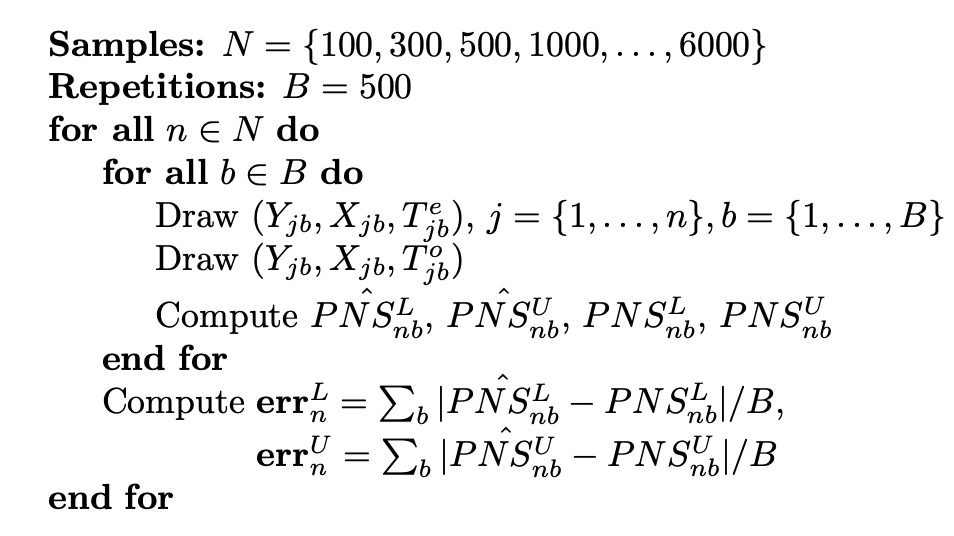
\includegraphics[width=6cm]{figures/sim.png}
\end{figure}


\end{column}%
\end{columns}


\end{frame}

%%%%Slide

\begin{frame}
[fragile]\frametitle{}

\begin{figure}[t]
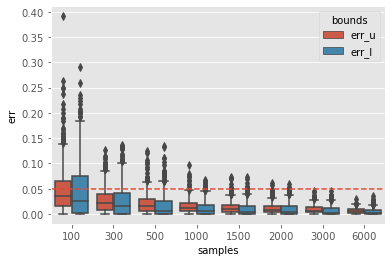
\includegraphics[width=6cm]{figures/simResults.png}
\end{figure}

\small{
\begin{itemize}

\item  \href{https://arxiv.org/abs/2210.05027}{Li, Mao and Pearl [2022]} derived sample size requirements to achieve an error rate of at most $\epsilon$, at $1-\alpha$ confidence-level. 

\item In the example above, their estimates give $N=6147$ for $\epsilon=0.05$ and $\alpha=0.05$.

\end{itemize}
}

\end{frame}



%%%%Slide

\begin{frame}
[fragile]\frametitle{}

\begin{center}


\begin{figure}[t]
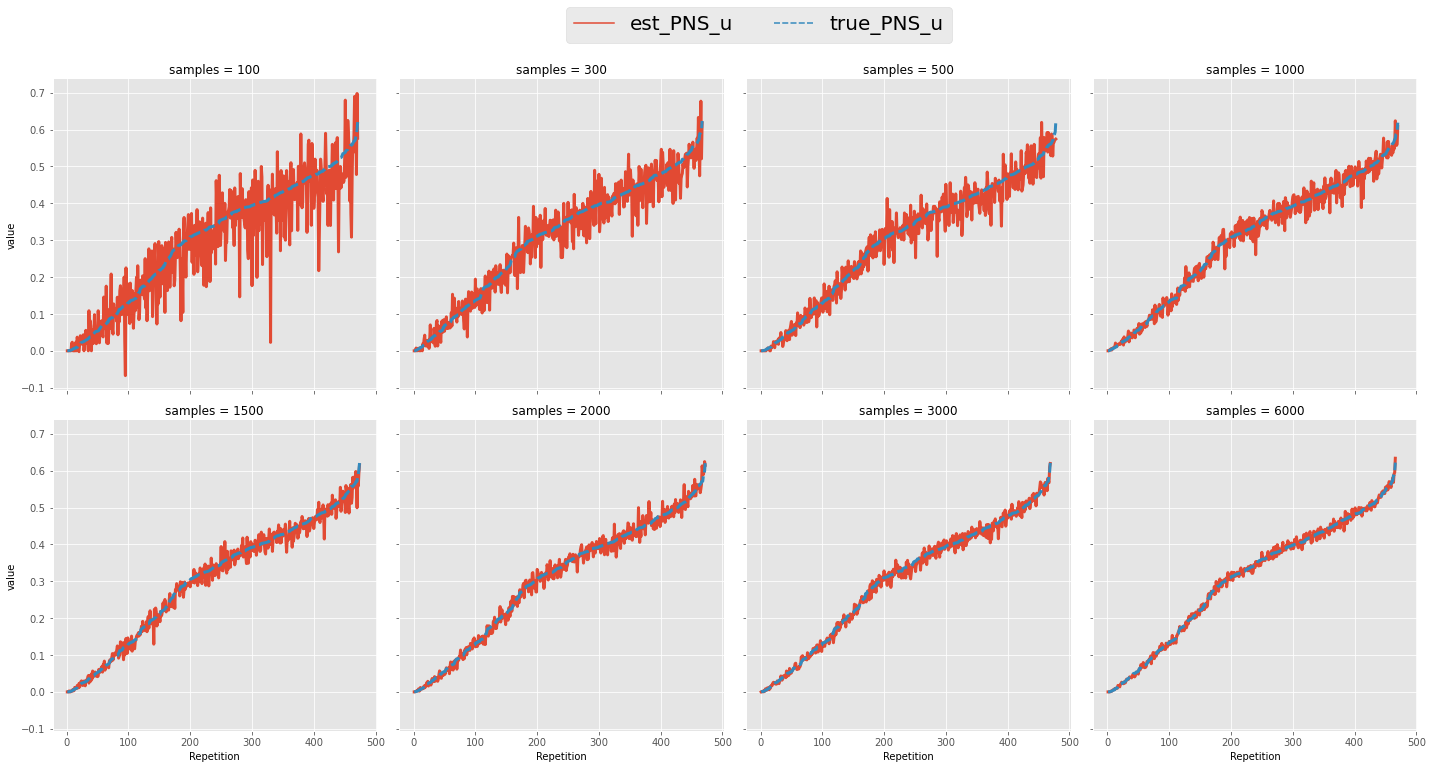
\includegraphics[width=7cm]{figures/pnsu.png}
\end{figure}


\begin{figure}[t]
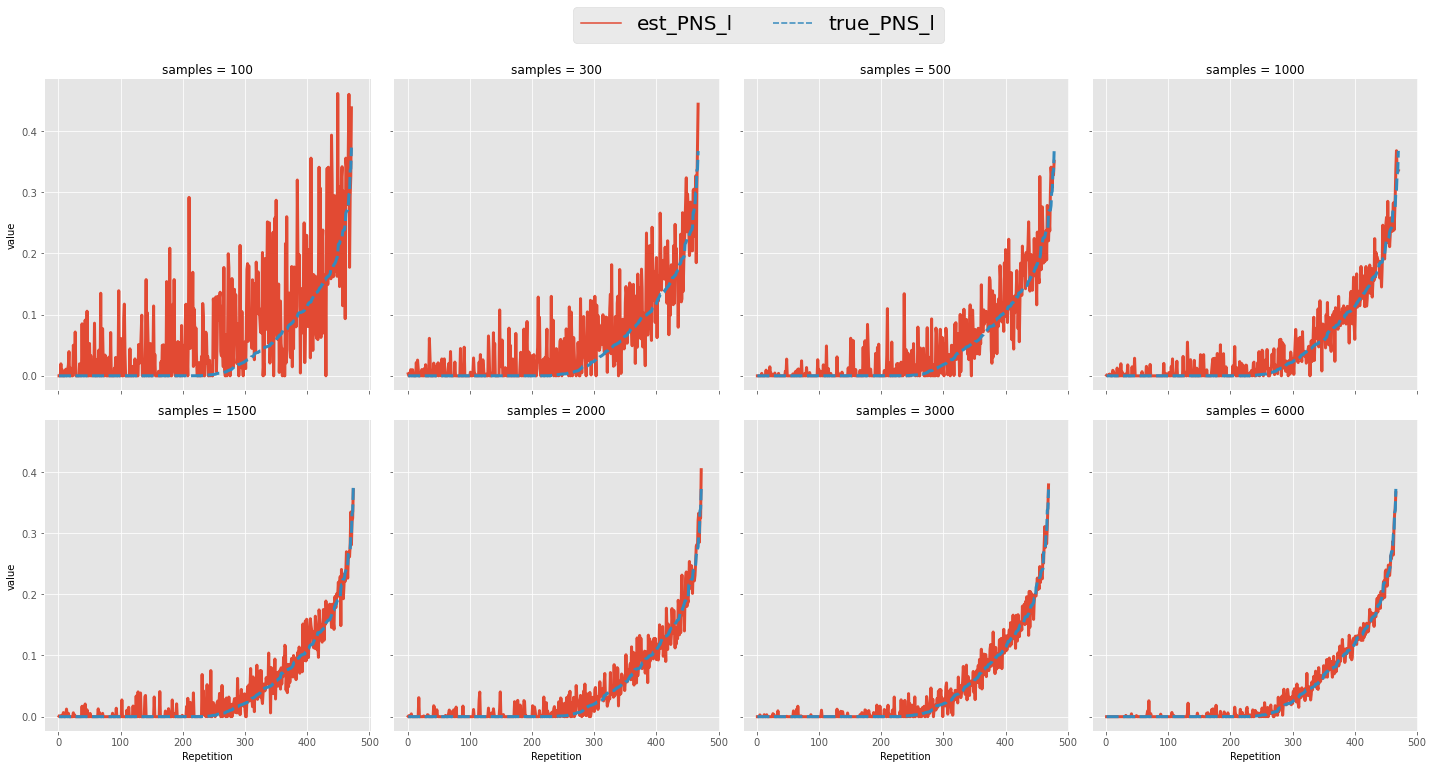
\includegraphics[width=7cm]{figures/pnsl.png}
\end{figure}

\end{center}




\end{frame}


%%%%Slide

\begin{frame}
[fragile]\frametitle{Work in Progress}

\begin{itemize}

\item \textbf{Goal}: Estimation of heterogenous benefit/harm effects with sharp empirical bounds. 

\begin{itemize}

\item Estimation procedure that provides lower error rates on upper/lower bounds, relative to baseline (based on independent estimation of observational and experimental distributions). 

\vskip10pt

\item Effectively deal with non-overlap issues between observational and experimental data.

\end{itemize}

\end{itemize}


\end{frame}


%%%%Slide

{
\setbeamercolor{background canvas}{bg=black}
\begin{frame}
\begin{center}

\Large{\textcolor{white}{Appendix}}

\end{center}
\end{frame}
}


%%%%Slide

\begin{frame}
[fragile]\frametitle{Monotonicity Violations}

\begin{itemize}

\small{

\item A \textbf{necessary condition} for monotonicity can be derived by checking that all arguments to the max function in the lower bound of $P(\text{harm}|X)$ are non-positive\footnote{$P(\text{harm}|X)$ bounds can be obtained from PNS and CATE using the relation derived in Slide 9.}: 

}
\scriptsize{

\begin{equation*}
\textrm{max} 
\left\{\!\begin{aligned}
&~~~~~~~~0 \\
& P(y_{t'} |x)-P(y_{t} |x)\\
& P(y |x)-P(y_{t} |x)\\
& P(y_{t'} |x)-P(y |x)\\
\end{aligned}\right\}
 \leq  P(\text{harm|}x) \leq \textrm{min}  
\left\{\!\begin{aligned}
&~~~~~~~~~~~~~~~~~~P(y_{t'} |x) \\
& ~~~~~~~~~~~~~~~~~~P(y'_{t} |x)\\
& ~~~~~~~~~~~P(y', t |x)+P(y, t' |x)\\
& P(y_{t'} |x)-P(y_{t} |x) +P(y, t |x)-P(y', t' |x)\\
\end{aligned}\right\}
\end{equation*}

}


\vskip5pt

\small{
\item From the above, we get

\begin{equation}\label{eq:1}
\text{Monotonicity} \Rightarrow P(y_{t} |x) \geq P(y|x) \geq P(y_{t'} |x) 
\end{equation}

}


\vskip5pt

\item By contrapositive, failure to satisfy the consequent of~\ref{eq:1} implies monotonicity violations. 

\vskip5pt


\item Given $P(Y, T |X)$, what are the hypothetical values of $P(y_{t} |x)$ and $P(y_{t'} |x)$ that entail violations to the inequality in~\ref{eq:1}?

\end{itemize}


\end{frame}


%%%%Slide

\begin{frame}
[fragile]\frametitle{}

\small{

\begin{itemize}


\item Interventional distributions are compatible with observational distributions under the following conditions\footnote{See Eq. 22 in  \href{https://ftp.cs.ucla.edu/pub/stat_ser/r271-A.pdf}{Jin Tian and Judea Pearl [2000]}.}:


\begin{align}\label{eq:2}
P(y, t |x) &\leq P(y_{t} |x)  \leq 1 - P(y', t|x) \\  
P(y, t' |x)  &\leq P(y_{t'} |x)  \leq 1 - P(y', t' |x). \nonumber 
\end{align}

\vskip5pt

Define the \textbf{compatible set} as $\mathcal{C}=\bigl\{ \big( P(y_{t} |x), P(y_{t'} |x) \big): \text{Ineq.(5)} \bigl\}$.

\vskip5pt

\item Example: Suppose we have the following observational and experimental data

\begin{itemize}

\item $P(t|x)=0.5$, $P(y|t, x)=0.5$, $P(y|t', x)=0.5$.

\item $P(y_t|x)=0.5$,  $P(y_{t'}|x)=0.5$.

\end{itemize}

\vskip5pt

Then, compatibility implies:

\begin{align*}
0.25 &\leq P(y_{t} |x)  \leq 0.75 \\
0.25  &\leq P(y_{t'} |x)  \leq 0.75.
\end{align*}


\end{itemize}

}
\end{frame}


%%%%Slide

\begin{frame}
[fragile]\frametitle{}

\small{

\begin{itemize}

\item Hence, incorporating the necessary condition for monotonicity (Ineq.~\ref{eq:1}), we get that interventional distributions must satisfy: 

\begin{align*}
0.50 &\leq P(y_{t} |x)  \leq 0.75 \\
0.25  &\leq P(y_{t'} |x)  \leq 0.50.
\end{align*}

\vskip5pt

\item Define the \textbf{necessary set} as  $\mathcal{N}=\bigl\{ \big( P(y_{t} |x), P(y_{t'} |x) \big): \text{Ineq.(4)}  \wedge   \text{Ineq.(5)} \bigl\}$.

\vskip5pt


\item Finally, define the \textbf{violation set} as $\mathcal{V} = \mathcal{C} \setminus \mathcal{N}$ -- i.e., $\mathcal{V}$  is composed of feasible values of the interventional distributions that would entail violations to monotonicity. 

\end{itemize}


\begin{figure}[t]
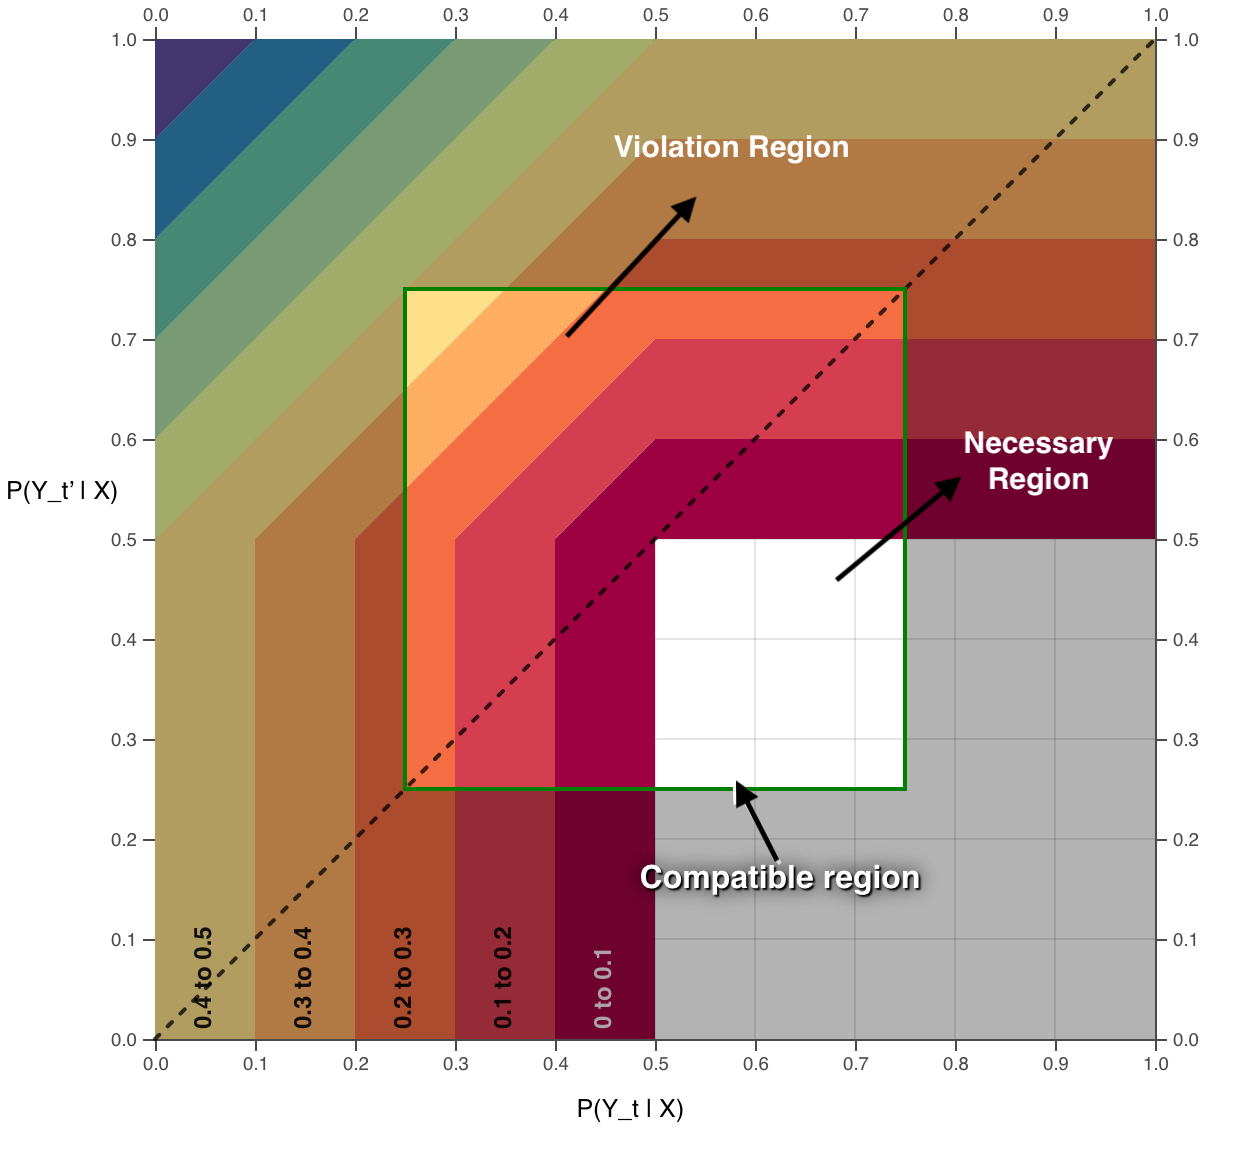
\includegraphics[width=4cm]{figures/v2.png}
\end{figure}


}

\end{frame}


\end{document}

